\documentclass{transcrypto}
\usepackage[utf8]{inputenc}
\usepackage[english]{babel}
\usepackage{amsmath, wasysym}
\usepackage[nottoc]{tocbibind}
\usepackage{colortbl}
%\usepackage[table]{xcolor}
\usepackage{dblfloatfix}
\usepackage{xeCJK}
\usepackage[titletoc]{appendix}
\usepackage{appendix}
\setcounter{MaxMatrixCols}{20}

\author{Tumma Manohar Sai\inst{1} \and Anugu Rakesh Reddy\inst{2} \and Goolla Abhijith\inst{3}}
\institute{Institute ID.: 11841170\\ Branch: Computer Science (CS) \\Email: \email{tummas@iitbhilai.ac.in} \and Institute ID.: 11840200\\ Branch: Electrical (EE) \\Email: \email{anugur@iitbhilai.ac.in} \and
           Institute ID.: 11840510\\ Branch: Computer Science (CS) \\Email: \email{goollaa@iitbhilai.ac.in} }
\title[\texttt{iacrtans} class documentation]{\publname}
\subtitle{CS553 Cryptography Term Paper}

\begin{document}
	\maketitle
	\keywords[\publname, ctp, ctp, LaTeX]{mCrypton, impossible differential, Lightweight cipher, cryptanalysis}
	
	\begin{abstract}
	In this term paper, we go through various aspects regarding mcrypton cipher and are explained thoroughly to gain a deeper understanding of the cipher. Mcrypton is the compact version of Crypton block cipher which is mainly used in the low-resources applications such as wireless devices. Firstly, We explained the encryption algorithm of mcrypton and the major transformation included in each round.   We searched over the web to find more about the cipher and found it vulnerable to quite a few number of attacks and we mentioned a few of the attacks. In this, we discussed the related-key impossible differential attack on 6-round and 9-round of mcrypton-96, the attack is quite similar for the mcrypton-128. We explained the complexity of the cipher using appropriate equations for data and time. Finally, We explained the uniqueness we felt during the entire research and knowledge we gained from the online resources in this time period and concluded the major points and applications related to mcrypton cipher.  
	\end{abstract}
	\newpage
	%\tableofcontents{}
	\newpage
	%\listoffigures
	%\newpage
	%\listoftables
	%\newpage
	\section{Introduction}
	As the demand for computing devices such as RFID tags and sensors in wireless sensor networks increases, Lightweight cryptography attains much more attention from the researchers. In the current scenario there are multiple lightweight block ciphers present. Examples such as SEA, mCrypton, PRESENT and new variants of KATAN, KTANTAN, etc.
	mCryption is a 64-bit lightweight block cipher.As it is known, it is a compact version of cryption. It is specifically designed to be used in low-cost and low-resources applications such as RFID tags and sensors in wireless sensor networks. It has 12 rounds with three key sizes of 64, 96, 128 bits. We represent a n bits cipher as mCrpton-n.\\
	
	
	At the time of introduction, It is shown that mCrypton is not vulnerable against differential and linear cryptanalysis. There are multiple attacks tried on mCrypton and some yield successful results such as meet in the middle(MITM) attack on round reduced mcrypton, biclique cryptanalysis and its variants such as Non-isomorphic biclique cryptanalysis, related-key rectangle attack, related-key impossible differential attack, collision attacks. In this paper, we mainly focus on related key impossible differential attack on round reduced mcrypton and Encryption algorithm of mcrypton.
	
	\section{Description of mCrypton}
	 mCrypton is a redesigned compact version of Crypton block cipher. mCrypton processes 64-bit data blocks, consisting of 16 nibbles by representing it as 4x4 matrix as follows.\\
	 \begin{center}
	 	$A = \begin{bmatrix}
	 	a_{0} & a_{1} & a_{2} & a_{3}\\
	 	a_{4} & a_{5} & a_{6} & a_{7}\\
	 	a_{8} & a_{9} & a_{10} & a_{11}\\
	 	a_{12} & a_{13} & a_{14} & a_{15}
	 	
	 	\end{bmatrix}$-
	 	{4x4 matrix consisting of 16 nibbles}
	 \end{center}
 mCrypton encryption/decryption is independent of its key size. It has a 12-round substitution -permutation structure. 

	
	\subsection{Round Description}
	Each Round consists of four major transformation steps as follows:
	\begin{itemize}
		\item \textbf{\textit{Step 1} : Nonlinear substitution $\gamma$:}
		
		
		We substitute nibble-wise using 4 S-boxes $S_{i}$ where i = 0, 1, 2, 3. The nibble located in row i and column j from above matrix A ( $a_{4xi + j}$) is passed through the s-box $S_{(i + j)mod 4}$.
		
		\item \textbf{\textit{Step 2} :  Bit permutation $\pi$:}
		
		
		We do bit wise permutation $\pi_i$ of column i. In column i for an input column a = $( a_0, a_1, a_2, a_3 )^t$ , we have $b_j$ = $\oplus_{k = 0}^3(a_{k}$$\bullet$$m_{(i+j+k)mod 4})$, 0 $\leq$ j $\leq$ 3, where $m_{0}$ = 1110, $m_{1}$ = 1101, $m_{2}$ = 1011, $m_{3}$ = 0111 are masking nibbles and ‘ $\bullet$ ’ represents And operation. $\pi$ transformation is an involution i.e, $\pi$ = $\pi^{-1}$. It has a differential branch of 4.
		\item \textbf{\textit{Step 3} :  Column-to-row transposition $\tau$
			:}
		
		Transpose of the matrix after step-2. Interchanging the nibble from ( i , j ) to ( j , i ).
		
		\item \textbf{\textit{Step 4} : Key addition $\sigma$:}
		
		For a round key $K_r$ = $K_{r,row(i)}$, i = 0, 1, 2, 3 is the round key in the ith row, B = $\sigma K_{r}$(A) is defined by $B_{row(i)}$ = $A_{row(i)}$ $\oplus$ $K_{r,row(i)}$, where i = 0, 1, 2, 3.
		
	\end{itemize}
	
	\begin{table}[H]
		\centering
		\begin{tabular}{|c|c|c|c|c|c|c|c|c|c|c|c|c|c|c|c|c|}
			\hline
			$x$ & 0 & 1 & 2 & 3 & 4 & 5 & 6 & 7 & 8 & 9 & $ a $ & $ b $ & $ c $ & $ d $ & $ e $ & $ f $ \\ \hline \hline
			$S_{0}(x)$ & 4 & $f$ & 3 & 8  & $d$ & $a$ & $ c $ & 0 & $b$ & 5 & $ 7 $ & $ e $ &  2  &  6  & 1 & 9 \\ \hline
			$S_{1}(x)$ & 1 & $c$ & 7 & $a$ & 6 & $d$ & 5 & 3 &$f$ & $b$ & 2 & 0 & 8 & 4 &  9 & $e$ \\ \hline
			$S_{2}(x)$ & 7 & $e$ & $c$ & 2 & 0 & 9 & $d$ & $a$ & 3 & $f$ & 5 & 8 & 6 & 4 & $b$ & 1 \\ \hline
			$S_{3}(x)$ & $b$ & 0 & $a$ & 7 & $d$ & 6 & 4 & 2 & $c$ & $e$ & 3 & 9 & 1 & 5 & $f$ & 8 \\ \hline
		\end{tabular}
		\caption{S-box}
	\end{table}
\begin{figure}[H]
	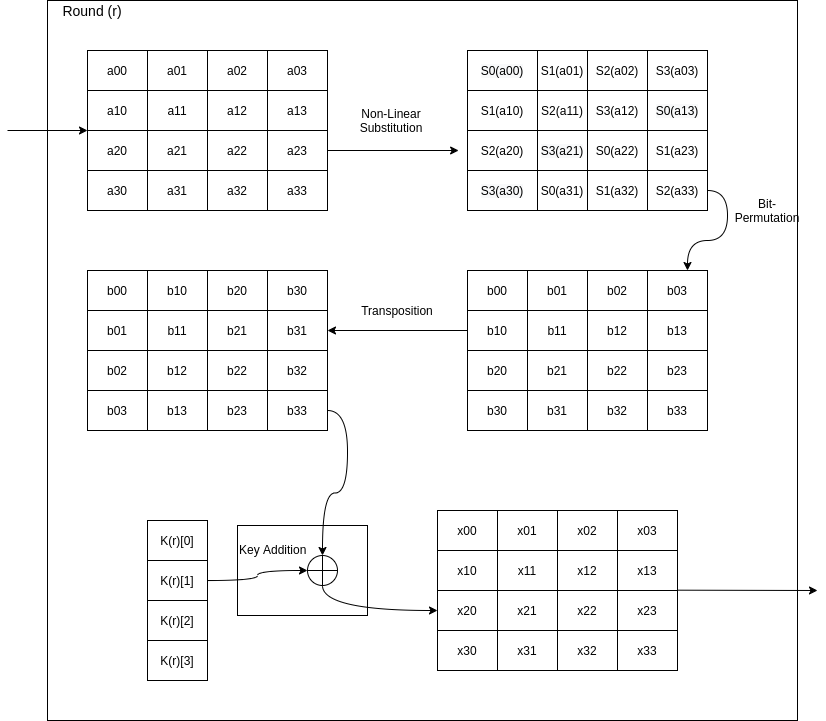
\includegraphics[width=1\linewidth]{Round.png}
\end{figure}
Initially U is the master key for encryption .It initially starts with the key addition $\sigma _{K_{0}}$. There will be 12 times of repetition of non linear substitution  followed by bit permutation, then followed by column to row transposition and lastly with key addition. Which is mathematically expressed asf $\rho _{K_i}$ = $\sigma _{K_i}$ $\bullet$ $\tau$ $\bullet$ $\pi$ $\bullet$ $\gamma$.This happens 12 times .At 12 th round it will be $\rho_{K_{12}}$ = $\sigma _{K_{12}}$ $\bullet$ $\tau$ $\bullet$ $\pi$ $\bullet$ $\gamma$. After this 12 rounds there will be one transformation for final output i.e , column to row transposition then bit permutation and followed by column to row transformation , which is mathematically represented as fp = $\tau$ o $\pi$ $\bullet$ $\tau$ . Now we can write the final output as fp $\bullet$ $\rho _{K_{12}}$ = $\tau$ $\bullet$ $\pi$ $\bullet$ $\tau$ $\bullet$  $\sigma _{K_{12}}$ $\bullet$ $\tau$ $\bullet$ $\pi$ $\bullet$ $\gamma$ . So the final result which we get is  fp $\bullet$ $\rho _{K_{12}}$ = $\tau$ $\bullet$ $\sigma _{K_{12}}$ $\bullet$ $\gamma$.


	\subsection{Key-Scheduling}
		\subsubsection{Key-scheduling of mcrypton-96:}
		\begin{figure}[H]
			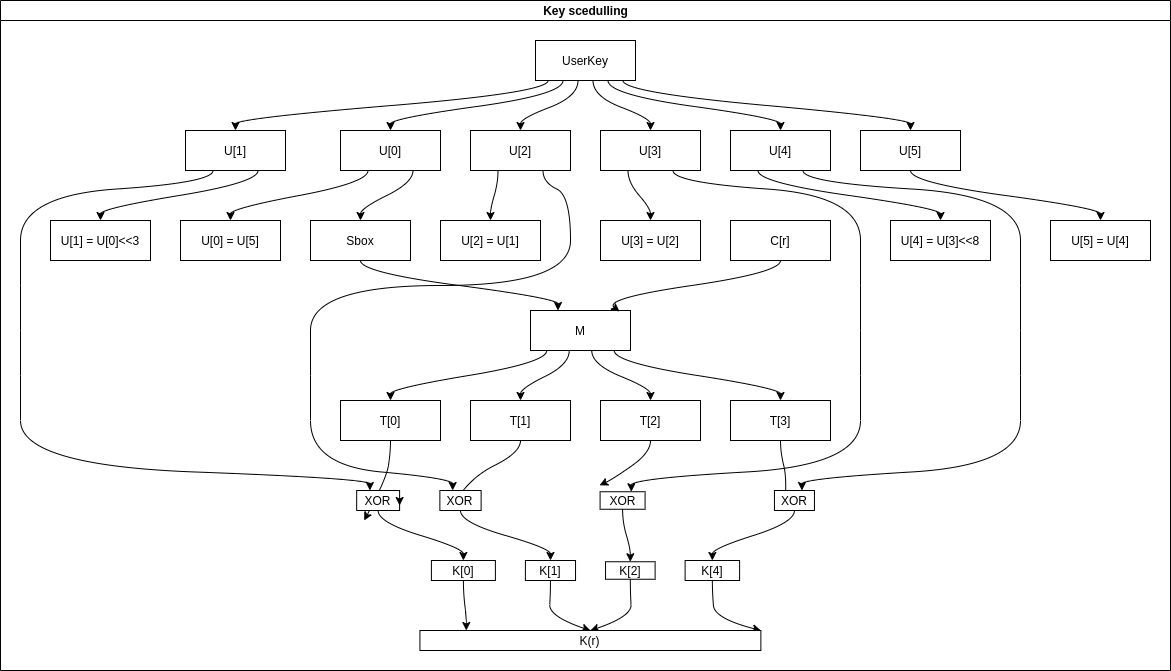
\includegraphics[width=1\linewidth]{KeyScedulling.png}
		\end{figure}
		 Initially $U = ( U[0], U[1], U[2], U[3], U[4], U[5])$ is the  96(16 * 6) Bit master key or user key. Now we have to generate round keys $K_{r}$, $0\leq r\leq 12$. Then we will calculate the round keys as below :\\\\
		$T \leftarrow S(U[0]) \oplus C[r], T_i \leftarrow T \bullet M_i$  (S(U[0]) is nibble wise sbox substitution)\\
		$i = 0, 1, 2, 3,$ $M_0$ =0xf000, $M_1$ =0x0f00, $M_2$ =0x00f0, $M_3$ =0x000f\\
		$K_r$ $\leftarrow$ $(U[1] \oplus T_0, U[2] \oplus T_1, U[3] \oplus T_2, U[4] \oplus T_3)$,\\
		$U \leftarrow (U[5], U[0]^{<<3}, U[1], U[2], U[3]^{<<8}, U[4])$ ($^{<<3}$ denotes bits are left rotated by 3 places)\\
		Round constant $C[r]$, $0\leq r \leq 12$ is a 16 bit number where most significant 4 bits are [0001, 0010, 0100, 1000, 0011, 0110, 1100, 1011, 1110, 0101, 1010, 0111, 1110, 1111] and all other are 0s for $S(U[0])$ 
			
		\subsubsection{Key-scheduling of mcrypton-128:}
		This is similar to 96-bit version except that master key or user key is initialised with $U = ( U[0], U[1], U[2], U[3], U[4], U[5], U[6], U[7])$ 128 bit number and the updating stage is as follows :\\
		$U \leftarrow (U[5], U[6], U[7], U[0]^{<<3}, U[1], U[2], U[3], U[4]^{<<8})$ 
	\subsection{S-Box and Bit-permutation Properties}
	\subsubsection{S-Box property :}
	We can see in our S-box $S_2 = S_0^{-1}$ and $S_3 = S_1^{-1}$
	\subsubsection{Bit-permutation property :}
	For a column $i$, $0\leq i\leq 3$ let $a$ be the input and $b$ be the output of bit permutation such that $b = \pi _{i}(a)$. Similarly for column $i'$, $0\leq i'\leq 3$ let $a'$ be the input and $b'$ be the output of bit permutation such that $b' = \pi _{i}(a')$. Now we have $f$, $0\leq f\leq 3$ such that $i' = (i + f)mod4$. Then  if $a'$ is circular shift of $n$ bits, $a' = a<<n$, $0\leq n\leq 3$, then the bits of $b'$  is also shift of bits of $b$ such that:\\
	
	$b'= 
	\begin{cases}
		b>>(s-f),& (s-f)\geq 0\\
		b<<(s-f)              & (s-f)<0
	\end{cases}$
	\section{Notations Used in mCryton}
	
	\begin{itemize}
		\item $x_r^{\gamma}$ : Values of matrix after Non-linear substitution trasformation in $r^{th}$ round.
		\item $x_r^{\pi}$ : Values of matrix after Bit-permutation trasformation in $r^{th}$ round.
		\item $x_r^{\tau}$ : Values of matrix after Column-to-tow transposition trasformation in $r^{th}$ round.
		\item $x_r^{\sigma}$ : Values of matrix after Key addition trasformation in $r^{th}$ round.
		\item $x_r^I$ : Input of matrix for $r^{th}$ round
		\item $x_r^O$ : Output of matrix from $r^{th}$ round..
		\item $K_{r, row(i)}$ : Key for round $r$ for $i^{th}$ row.
	\end{itemize}

	\section{Various attacks on mCrypton}
	Even though designers of mcrypton cipher showed secure against differential and linear cryptanalysis, there are still quite a few attacks which are successful. A related-key rectangle attack on 8-rounds mcrypton-128 has been successful with a success rate of 0.94 with the data, time and memory complexities of about $2^{46}$ plaintexts, $2^{46}$ encryptions, and 5x$2^{48}$ bytes, respectively. In this paper, we discuss in depth the related-key differential impossible attack on mcrypton.\\
	
	
	Related-key attacks use the information from the past encryption data using related-keys. In this attack, the attacker exploits the differential relations with probability zero in two encryptions under two related keys. By utilizing the low diffusion in the key schedule of mcrypton, we attack with two related-key differential attacks on 9 rounds of mcrypton-96 and mcrypton-128. It takes $2^{59.9}$ chosen plaintexts, time complexity of $2^{74.9}$ encryptions for mcrypton-96 using this attack. Similarly, we even got better results in case of mcrypton-128 with $2^{59.7}$, $2^{66.7}$ data and time complexities respectively.
	
	
	\section{Related-key differential impossible attack:
	}
	In this, we provide a brief discussion of 6-round related-key differential impossible and its consequent attack on 9-round mcrypton-96 and also a similar procedure on mcrypton-128.
	\subsection{6-round related-key impossible differential of mcrypton-96:}
	We choose the difference between two related keys $K$ and $K^1$ as follows:\\
	$$\Delta K = K \oplus K^1 = (0000|0000|0000|a000|0000|0000).$$
	Based on the key schedule of mcrypton-96, the subkey differences in the first 9 rounds are shown below table 1.
	\begin{table}[H]
		\centering
		\begin{tabular}{c c c c c}
			\hline
			Round$(i)$ & $\Delta K_(i,row(0))$ & $\Delta K_(i,row(1))$ & $\Delta K_(i,row(2))$ & $\Delta K_(i,row(3))$\\
			\hline
			0 & (0000) & (0000) & ($a$000) & (0000)\\
			1 & (0000) & (0000) & (0000) & (00$a$	0)\\
			2 & (0000) & (0000) & (0000) & (0000)\\
			3 & (0000) & (0000) & (00$b$0) & (0000)\\
			4 & $(a000^{<<11})$ & (0000) & (0000) & (0000)\\
			5 & (0000) & $(a000^{<<11})$ & (0000) & (0000)\\
			6 & (0000) & (0000) & $(a000^{<<11})$ & (0000)\\
			7 & (0000) & (0000) & (0000) & $(a000^{<<3})$\\
			8 & (0000) & (0000) & (0000) & (0000)\\
			9 & ($b'$000) & (0000) & (0000) & (000$b''$)\\
			\hline
			 
		\end{tabular}\\
	$a$, $b$ and at least one of $b'$ and $b''$ are non-zero nibble differences.
	\caption{Subkey differences in 9 rounds of mCrypton-96}
	\end{table}

	A 4.5-round related-key differential with probability 1 from forward direction and a 1.5-round related-key differential with probability 1 from the reverse direction where the intermediate differences contradict each other forms the 6-round related-key impossible differential as.
	$$\Delta x_1^{\pi} = (0000|0000|000a|0000) \nrightarrow \Delta x_7^{\gamma} = (0000|0000|????|????),$$
	\begin{figure}
		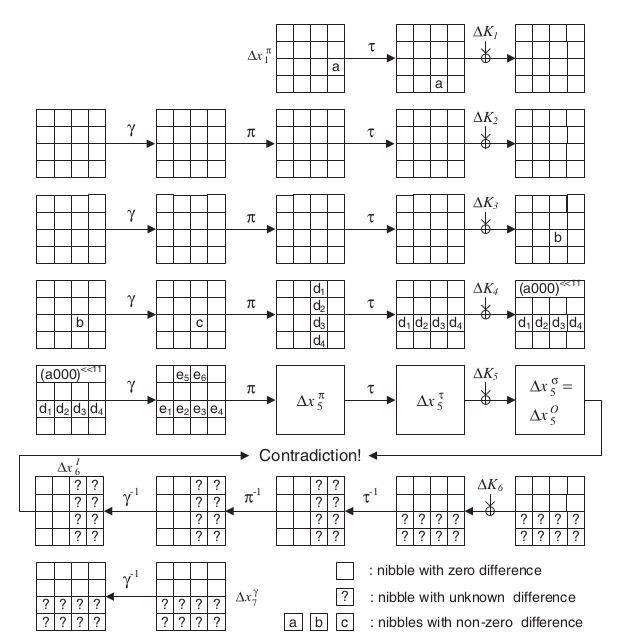
\includegraphics[width=1\linewidth]{1.png}
		\caption{6-Round related-key impossible differential of mCrypton-96.}
	\end{figure}
	where $a$ is a non-zero value and ‘?’ denotes any value. The related-key impossible differential is
	shown in Figure 1 in which the boxes with ‘$a$’, ‘$b$’ or ‘$c$’ in them refer to nibbles with non-zero
	difference, whereas the boxes with ‘?’ in them refer to nibbles with unknown difference, and white
	boxes refer to nibbles with zero difference.
	\textbf{First 4.5-round differential is as follows:}\\
	Here $\Delta$ $x_1^{\pi}$ is cancelled with $\Delta$ $K_1$. Since $\Delta$ $K_2$ = 0, $\Delta$ $x_2^I$ remains the same until the third round. 
	Thus $$\Delta x_4^I = \Delta K_3=(0000|0000|00b0|0000)$$.
	In the round 4, $\gamma$ converts row (00b0) to (00c0) as shown below and the $\pi$ transformation converts row (00c0) to column ($d_1$, $d_2$, $d_3$, $d_4$).After the key addition in round 4, we will get $\Delta x_4^o = ((a000)^{<<11}|0000|d_1 d_2 d_3 d_4|0000)$. Thus, we are sure that in $\Delta$ $x_5^{\gamma}$ at least one of the columns 0 and 3 has only one non-zero nibble. Consequently, after the application of in round 5, the column with 1 non-zero nibble is converted into a column with 3 or 4 non-zero nibbles. Hence, in $\Delta x_5^{\tau}$ at least one of the two rows 0 and 3 has 3 or 4 non-zero nibbles. Since $\Delta K_5$ is zero in rows 0 and 3, this property holds for $\Delta x_5^o$.
	
	\textbf {Second 1.5-round differential as follows:}\\
	The second differential ends at round-7 after the substitution having a value $$\Delta x_7^{\gamma} = (0000|0000|????|????)$$ as shown. However $\Delta K_6$ is zero in the first two rows, $\Delta x_6^{\tau}$ will be zero in these two rows. Hence, when we do the differential from the reverse direction of $\tau^{-1}$, $\pi^{-1}$ and $\gamma^{-1}$, we have the value $$\Delta x_6^{I} = (00??|00??|00??|00??)$$. We can conclude $\Delta x_6^{I}$ equal to  $\Delta x_5^{o}$ . However, $\Delta x_5^{o}$ has 3 or 4 non-zero values in at least one of its rows, while $\Delta x_6^{I}$ does not have more than 2 non-zero nibbles in all rows; this is the contradiction. We mention that since $\Delta K_6$ has non-zero nibbles in its third row (which is row 2 with the convention), one of the rows with the form (????) in $\Delta x_7^{\gamma}$ must lie in the third row i.e, row 2. Therefore, there are only three possible cases to put two rows with the form (????) in $\Delta x_7^{\gamma}$.
	\subsection{AN ATTACK ON 9-ROUND mCRYPTON-96}
	\begin{figure}[H]
		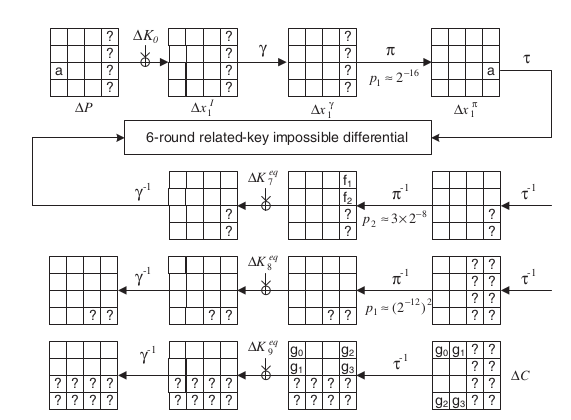
\includegraphics[width=1\linewidth]{2.png}
		\caption{Related-key impossible differential attack on 9-round mCrypton-96.}
	\end{figure}
	Here, we use the above 6-round related-key distinguisher to do the related-key impossible differential attack on 9-round mcrypton-96. The attack is as follows in the given picture.
	
	To reduce the time complexity from the rounds 7 to 9, we change the order of round structure from $\sigma$, $\tau$, $\pi$ to $\tau$, $\pi$, $\sigma$. Since we changed the order, the equivalent key changes for each round as $K_i^{eq}$ is $\pi$ transformation of $\tau (K_i)$ i.e, $\pi (\tau (K_i))$. In our attack, we have 16 related keys $K^{0}$.......$K^{15}$ which have a change at nibble 15. We suppose that the relation between these keys is such that $K_i \oplus K_j =(0000|0000|0000(i \oplus j)000|0000|0000),i, j = 0,1,...,15$. We are assuming that the attacker has access to 16 encryption modules $E_0$,..., $E_15$ where the encryption key of $E_j$ is $K_j$ , j =0,1,...,15.
	
	Our attack uses related keys with the subkey differences which are available in Table 1. The value a can be chosen by the attacker, but the values of b’ and b’’ in $\Delta K_9$ that are results of application of S-boxes are unknown. However, b’ and b’’ can take 24 values each, thus Keq 9 can take only 24 values in columns 0 and 3 each. We remind that since the branch number of is 4, knowing 2 nibbles of ($\pi (b’000)^t$ ) uniquely determines $b^{'}$ and the other 2 nibbles of ($\pi (b’000)^t$ ). Also the same property holds for ($\pi (000b’’)^t$ ). Hence, if we consider the 4-nibble quantity of $K_{9,(0)}^{eq} | K_{9,(4)}^{eq} | K_{9,(3)}^{eq} | K_{9,(7)}^{eq}$, this 16-bit quantity takes only 28 values. The attacker precomputes these values and prepare a table H with 28 rows such that each row has an index equal to one of these values. The table H will be filled in step 2 of the attack procedure. 
	
	As a precomputation stage, prepare 15 tables $T_a$,a=1,...,15 as follows. For all the $2^{16}$ possible pairs of values of ($x_{1,col(3)}^{\pi}$, $x’_{1,col(3)}^{\pi}$) that have the difference $\Delta$ $x_{1,col(3)}^{\pi} =(00a0)^t$ , partially decrypt these values to obtain the 4-nibble values ($x_{1,col(3)}^I$, $x’_{1,col(3)}^I$). Store the obtained pairs in table $T_a$ indexed by their differences. 
	
	The attack procedure is as follows:
	\begin{enumerate}
		
	
	\item Take 2n structures $S_m$,m =0,1,...,2n −1 of plaintexts such that each structure contains $2^{20}$ plaintexts of the form: $$P =(x_0x_1x_2 \alpha _3|x_4x_5x_6\alpha _7|\alpha _8x_9x_{10}\alpha _{11}|x_{12}x_{13}x_{14}\alpha _{15})$$, where the 5 nibbles $\alpha_3$,$\alpha_7$,$\alpha_8$,$\alpha_{11}$ and $\alpha_{15}$ take all the possible values, and the bytes of the form $X_x$ are fixed values in each structure. It is obvious that each structure proposes about $2^{40}$ ordered plaintext pairs with the difference $P =(000?|000?|?00?|000?)$.
	\item For $m = 0,1,...,2n -1$: 
	
	For $j =0,1,...,15$ Ask for the encryption of the structure $S_m$ under $K^j$, and store all the ciphertexts in a table $H_j$ indexed by their value in the 4 nibbles 4, 5, 8 and 9.Table $H_j$ has $2^{16}$ rows, thus after the encryption of a structure, on average $2^{20}$/$2^{16}$ =$2^4$ ciphertexts lie in each row of each table $H_j$ . Hence, if C is a ciphertext in a row of $H_i$ , and C is a ciphertext in a row with the same index in another table $H_j$,i, j =0,1,...,15, then $(C,C^{'})$ is a ciphertext pair with zero difference in nibbles 4, 5, 8 and 9. Thus we can extract about 16$P_2$ x$2_{16}$x$2_4$x$2^4$ $\approx$ $2^{31}$ 6-tuples $(P, C, i, P^{'}, C^{'}, j)$ from each structure, where $C$ is the ciphertext of the plaintext $P$ under the key $K_i$ , and $C^{'}$ is the ciphertext of the plaintext $P^{'}$ under $K_j$. For each of these pairs ($C$,$C^{'}$ ) check whether the difference value in nibbles 0, 1, 12 and 13 is equal to one of the $2^8$ possible indexes of table $H$ (explained above). The probability of this event is $2^{-8}$, thus about $2^31$x$2^{−8}$ = $2^{23}$ of such pairs exist. Now consider the 6-tuple $(C, P, i, C^{'}, P^{'}, j)$ that satisfies this condition and check if $P(8) =i \oplus j$ or not. If this condition is satisfied, the plaintext pair $(P, P^{'})$ has the same difference $i$ $\oplus$ $j$ as the related keys $K^i$ and $K^j$ have in the nibble 12 (in Figure 2 this difference has been shown by a). Put such 6-tuples in the row $\Delta C_0|\Delta C_1|\Delta C_{12}|\Delta C_{13}$ of table H. The probability of the latter condition is $2^{-4}$, thus, for each structure we expect to add about $2^{23}$x$2^{-4}$=$2^{19}$ 6-tuples into table H. As described above, this table has $2^8$ rows, hence we expect from each structure to add on average $2^{19}$/$2^8$ =$2^{11}$ proper 6-tuples into each row of H. Thus by examining all the $2^n$ structures, we store $2^{n+11}$ proper 6-tuples in each row of table H. 
	\item Guess the value of $\Delta$ $K_{9,col(0,3)} ^{eq}$ (recall that although $\Delta$ $K_{9,col(0,3)} ^{eq}$ is a 32-bit value, but according to the key schedule construction it only takes $2^8$ possible values corresponding to the indexes of table $H$). For each guess, obtain the ciphertext pairs $(C,C^{'})$ that after the partial decryption through  and equivalent key addition result in the difference $\Delta x_{9,row(0,1)} ^{eq}$ =0000|0000. It is obvious that these pairs are those stored in the row with the index $K_{9,(0)}^{eq}$|$K_{9,(4)}^{eq}$|$K_{9,(3)}^{eq}$|$K_{9,(7)}^{eq}$ in table H. Thus for each guess, we obtain about $2^{n+11} pairs (6-tuples)$. 
	\item Guess a 16-bit value and consider it as $\Delta K_{9,row(2)}^{i,eq}$. Notice that since $\Delta K_9^{eq}$ is fixed in this step, and for each of the $2^{n+11}$ plaintext pairs the values of $i$ and $j$ are also known, we immediately obtain only one value for $\delta K_{9,row(2)}^{j,eq}$. Based on this knowledge, for each ciphertext pair $(C,C^{'})$, partially decrypt $C$ using $\Delta K_{9,row(2)}^{i,eq}$ and $C’$ using $\Delta K_{9,row(2)}^{i,eq}$ through one round. Keep only the pairs for them $\Delta x_{8,col(2)}^{\sigma}$ is zero in the first 3 nibbles and non-zero in the last nibble. The probability of this condition is about $2^{-12}$, thus we expect about $2^{n+11}\times2^{-12}$ = $2^{n-1}$ pairs remain. 
	\item Guess a 16-bit value and consider it as $\Delta K_{9,row(3)}^{i,eq}$. For each of the $2^{n-1}$ remaining ciphertext pairs $(C,C^{'})$, partially decrypt $C$ using $\Delta K_{9,row(3)}^{i,eq}$ and $C’$ using $\Delta K_{9,row(3)}^{i,eq}$ through one round. Keep the pairs for them $\Delta x_{8,col(3)}^{\sigma}$ is zero in the first 3 nibbles and non-zero in the last nibble. The probability of this condition is about $2^{-12}$, thus we expect about $2^{n-1}\times 2^{-12}$ =$2^{n-13}$ pairs remain. 
	\item Guess the 8-bit value of $K_{8,(14,15)}^{i,eq}$ (recall from Table 1 that $\Delta K_8$ =0, thus $\Delta K_8^{eq} =0$). For each guess partially decrypt all the $2^{n-13}$ remaining pairs through one round. Keep only the pairs for them $\Delta$ $x_{7,col(3)}^{\sigma}$, in its 2 out of the 3 nibbles 3, 7 and 15, is equal to $K_{7,col(3)}^{eq}$ = $\pi(\tau(((i \oplus j)000)^{<<3})$. Let us denote this known 4-nibble difference by ($ f_1 f_2 f_3 f_4$). Thus $\Delta x_{7,col(3)}^{\sigma}$ can take 3 desired forms with probability of about 3$\times$$2^{-8}$ $\approx$ $2^{-6.4}$. Thus we expect about $2^{n-13}\times2^{-6.4}$ = $2^{n-19.4}$ pairs remain. 
	\item Initialize a list L of all the $2^{16}$ possible values of $K_{0,col(3)}^{0}$ (from Table I it is obvious that $K_{0,col(3)}^{0}$ = $K_{0,col(3)}^{i}$,i =1,...,15). 
	\item For each of the $2^{n-19.4}$ remaining 6-tuples, compute $\Delta P_{col(3)}$ and access the row with the same index in table $T_{i \oplus j}$ . For each pair $(x, y)$ in that row, remove from L the value $x$ $\oplus$ $P_{col(3)}$ and $y \oplus P_{col(3)}$. Thus the probability that a subkey $K_{0,col(3)}^{0}$ is removed by a remaining pair is $2^{-15}$. After trailing all the $2^{n-19.4}$ pairs, if L is not empty, return the values in L along with the guess of $K_{9,row(2,3)}^{i,eq}$|$K_{8,(14,15)}^{i,eq}$.
	\end{enumerate}
	
	\section{Algorithm Specifications and Hardware implementation compared to other block ciphers}
	\subsection{Algorithm specifications}
	\begin{table}[H]
		\centering
		\begin{tabular}{|c|c|c|c|}
			\hline
			\textbf{Block cipher} & \textbf{Key size(bit)} & \textbf{Block size(bit)} & \textbf{Round No.}\\
			\hline
			CLEFIA &128-bit &128,192,256 & 18,22,26 \\
			\hline
			PRESENT & 80,128 &64-bit &31 \\
			\hline
			HIGHT & 128-bit & 64-bit& 32\\
			\hline
			mCrypton & 96,128 &64-bit & 12\\
			\hline
		\end{tabular}
	\end{table}
	\subsection{Hardware implementation}
	 mCrypton is designed by following the overall architecture of Crypton but with redesign and simplification of each component function to enable much compact implementation in both hardware and software. A simple hardware implementation of mCrypton is also presented to demonstrate its suitability to our target applications. A prototype implementation based on the straightforward 1 cycle/round architecture just requires about 3500 to 4100 gates for both encryption and decryption, and about 2400 to 3000 gates for encryption only (under 0.13μm CMOS technology). The result shows that the hardware complexity of mCrypton is quite well within an economic range of low-cost RFID tags and sensors. A more compact implementation under development promises that further size reduction around 30\% could be achievable using the 5 cycles/round architecture.
	\begin{table}[H]
		\centering
		\begin{tabular}{|c|c|c|c|}
			\hline
			\textbf{Block cipher} & \textbf{Clock cycles} & \textbf{Area
				GE} & \textbf{Throughput
				Kbps}\\
			\hline
			CLEFIA 128 &18 &5979 &711.11 \\
			\hline
			CLEFIA 192 &22 &8536 &581.8 \\
			\hline
			CLEFIA 256 &26 &8482 &492.3 \\
			\hline
			PRESENT 80 &32 &1570 & 200 \\
			\hline
			PRESENT 128&32 &1884 & 200 \\
			\hline
			HIGHT &34 &2608 &188.2 \\
			\hline
			mCrypton 96 &13 &3789 &492.3 \\
			\hline
			mCrypton 128&13 & 4108&492.3 \\
			\hline
		\end{tabular}
	\end{table}
	\section{Complexity of the attack}
	The target subkey space includes $K_{9,row(2,3)}^{i,eq}$|$K_{8,(14,15)}^{i,eq}$|$K_{0,col(3)}^{0}$, with the cardinality of $2^{56}$. The value of i and consequently $K_{9,row(2,3)}^{i,eq}$ differ for different 6-tuples, so one may think the target subkey space is greater than 56 bits. But, based on the round key differences shown in Table 1, and the fact that for an invertible 4-bit S-box, on average one pair of nibbles satisfy a specific input difference and output difference, the attacker can obtain on average one value $K_{9,row(2,3)}^{0,eq}$ corresponding to each pair ($K_{9,row(2,3)}^{i,eq}$, $K_{9,row(2,3)}^{j,eq}$) guessed in steps 4 and 5. So we can consider the target subkeys as $K_{9,row(2,3)}^{0,eq}$|$K_{8,(14,15)}^{0,eq}$|$K_{0,col(3)}^{0}$. In step 8, the probability that one of the $2^{56}$-1 wrong subkeys survives the filtration is $(1-2^{-15})^{2^{n-19.4}}$ . Considering the fact that this procedure repeats for each of the $2^8$ possible values of $\Delta$ $K_{9,col(0,3)}^{eq}$, if we accept that only 1 subkey remains, then from equation $2^8\times(2^{56}-1)\times(1-2^{-15})^{2^{n-19.4}}$ =1, n will be 39.9. Thus the attack requires $2^{n+20} = 2^{59.9}$ chosen plaintexts. 
	
	In step 2, to get the qualified pairs, we first store the ciphertexts of each structure in a hash table indexed by the nibbles 4, 5, 8 and 9 of ciphertext. Then, we check two conditions on the $2^{n+31}$ pairs to embed about $2^{n+19}$ proper pairs in table H. The time complexity of this step is $2^{n+20}x16=2^{63.9}$ encryption for obtaining the ciphertexts, and about $2^{n+31}$ = $2^{70.9}$ memory accesses to check the two conditions. This step also requires $1/8\times2^{n+19}\times(4x64+8)$ $\approx$ $2^{63.9}$ bytes of memory for storing the $2^{n+19}$ proper 6-tuples in table $H$.
	
	 According to the attack procedure, the time complexity of the other steps in terms of encryption units (unless MA is mentioned for memory accesses) is computed as follows: \\
	 Step 3:\\
	 $2^{n+11}x2^8$ = $2^{58.9}$  MA \\
	 Step 4: \\
	 2 $\times$ 1/9 $\times$ 1/4 $\times$ $2^{n+11} \times$ $2^{8+16}$ $\approx$ $2^{70.7}$ \\
	 Step 5: \\
	 2 $\times$ 1/9 $\times$ 1/4 $\times$ $2^{n-1} \times$ $2^{24+16}$ $\approx$ $2^{74.7}$ \\
	 Step 6: \\
	 2 $\times$ 1/9 $\times$ 1/4 $\times$ $2^{n-13} \times$ $2^{40+8}$ $\approx$ $2^{70.7} $\\
	 Step 7: \\
	 2 $\times$ $2^{n-19.4}$ $\times$ $2^{48}$ = $2^{69.5}$ \\
	 Thus, the dominant part of time complexity is related to steps 4, 5 and 6 which is about $2^{70.7}$ + $2^{74.7}$ + $2^{70.7}$ $\approx$ $2^{74.9}$ encryptions. Compared with the memory required for step 2, the memory complexity of the other steps is negligible.
	
	 The procedure of the above attack is similar for mcrypton-128 where 128 is the key size.
	 
	
	
	\section*{Brownie Points}
	\begin{itemize}
		\item Visuaizations like Encryption algorithm and Keyschedulling were added for better Understanding.
		\item Properties like S-Box and Bit-permutation is analyzed.
		\item Over all the attacks, the complexities data, time and memory of related key impossible differencial attack on mCrypton has the least values. Therefore it is more vulnerable to this attack than any other.
		\item According to the theoretical observations, as most of the ciphers which are SPN networks which are designed for resource constrained devices are vulnerable to differential and linear cryptanalysis, but mcrypton was secured against those attacks.
		\item Comparision with other Block ciphers in Hardware implementation.
	\end{itemize}
	\section*{Conclusion}
	mCrypton as the name suggests, is a miniature of crypton, a compact version of crypton block cipher. It is mainly designed for lightweight cryptography for resource-constrained, low-power consumption and compact size. If we talk about practical usage, It provides 3 key sizes for better flexibility for cost-security trade-offs which is for minimal, moderate and standard securities, respectively. If we consider the hardware architecture, it is one of the best available ciphers and the software implementation was also quite simplified from the cipher crypton which is inline with the hardware architecture. In this, we learned how lightweight cryptography came into play, when there was demand for resource-constrained devices. Also mentioned a few ciphers which are currently in the market. We briefly discussed mCrypton which is the compact version of Crypton and the encryption algorithm by going in depth details of each sub-round and also explaining the Key-scheduling.  We mentioned a few attacks on mCrypton, in which we discussed the Related-key impossible differential attack on 6-round and 9-round mCrypton-96 and showed the detailed explanation at each round. We found the complexities of the attack and discussed the hardware implementation. We also mentioned a few unique points of mCrypton compared to other ciphers.
	
	\newpage
	\begin{thebibliography}{9}
		\bibitem{1}
		Bono, S., Green, M., Stubblefield, A., Juels, A., Rubin, A., Szydlo, M.: Security analysis of a cryptographically-enabled RFID device. In: 14th USENIX Security Symposium, Baltimore, Maryland (July-August 2005)
		\bibitem{2}
		Campbell, R.H., Al-Muhtadi, J., Naldurg, P., Sampemane, G., Mickunas, M.D.: Towards Security and Privacy for Pervasive Computing. In: Okada, M., Pierce, B.C., Scedrov, A., Tokuda, H., Yonezawa, A. (eds.) ISSS 2002. LNCS, vol. 2609, pp. 1–15. Springer, Heidelberg (2003)
		\bibitem{3}
		.Feldhofer, M., Dominikus, S., Wolkerstorfer, J.: Strong authentication for RFID systems using the AES algorithm. In: Joye, M., Quisquater, J.-J. (eds.) CHES 2004. LNCS, vol. 3156, pp. 357–370. Springer, Heidelberg (2004)
		\bibitem{4}
		Garfinkel, S.L., Jeuls, A., Pappu, R.: RFID privacy: An overview of problems and proposed solutions. IEEE Security \& Privacy, 34–43 (May/June 2005)
		\bibitem{5}
		Lim KH, Korkishko T. mCrypton—a lightweight block cipher for security of low-cost RFID sensors. WISA 2005, Lecture Notes in Computer Sciences, vol. 3786. Springer: Berlin, 2006. 
		\bibitem{6}
		VHDL implementation of mCrypton
		\href{https://github.com/huljar/mcrypton-vhdl}{github.com/huljar/mcrypton-vhdl}
		\bibitem{7}
		mCrypton - A Lightweight Block Cipher for Security of Low-Cost RFID Tags and Sensors
		\href{https://www.semanticscholar.org/paper/mCrypton-A-Lightweight-Block-Cipher-for-Security-of-Lim-Korkishko/7fca481caa31976a3c07989a295e804c1eeb9c76}{www.semanticscholar.org/paper/mCrypton-A-Lightweight-Block-Cipher-for-Security-of-Lim-Korkishko}
		\bibitem{8}
		Lightweight Block Ciphers
		\href{https://www.cryptolux.org/index.php/Lightweight_Block_Ciphers#mCrypton}{www.cryptolux.org/index.php/Lightweight\_Block\_Ciphers}
		\bibitem{9}
		\href{https://www.swmath.org/software/9729}{www.swmath.org/software/9729}
		\bibitem{10}
		Related-key impossible differential cryptanalysis on Crypton and Crypton v1.0
		\href{https://www.researchgate.net/publication/241181550_Related-key_impossible_differential_cryptanalysis_on_Crypton_and_Crypton_v10}{/www.researchgate.net/publication/241181550\_Related-key\_impossible\_differential\_cryptanalysis\_on\_Crypton}
		\bibitem{11}
		Biclique Cryptanalysis on the Full Crypton-256 and mCrypton-128
		\href{https://www.hindawi.com/journals/jam/2014/529736/}{hindawi.com/journals/jam/2014/529736/}
	\end{thebibliography}
\end{document}